\documentclass[border=6pt]{standalone}
\usepackage{tikz}
\usetikzlibrary{arrows.meta,positioning,calc,shapes.geometric,fit,backgrounds,patterns,matrix,decorations.pathreplacing}
\begin{document}
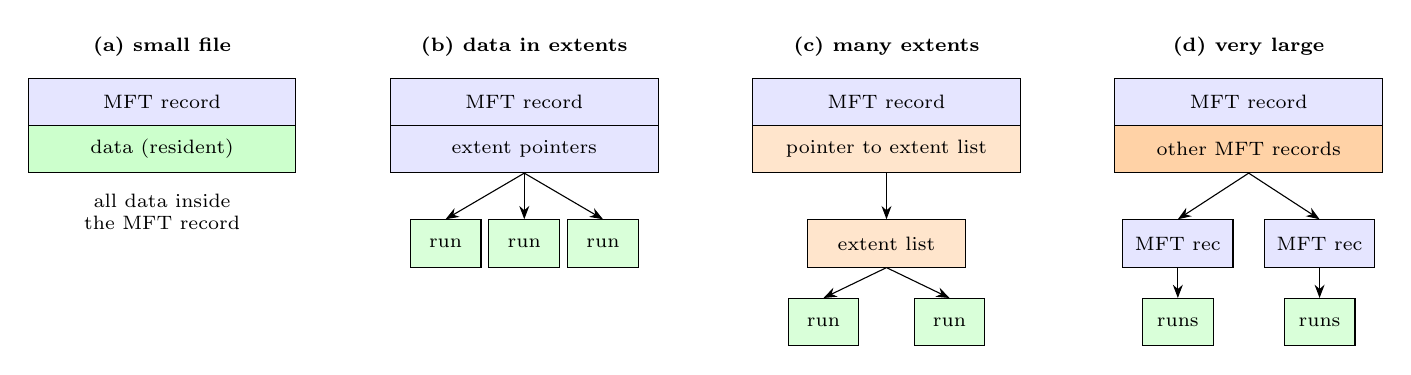
\begin{tikzpicture}[>=Stealth,font=\small]
\tikzstyle{m}=[draw,minimum width=3.4cm,minimum height=0.6cm,font=\scriptsize,fill=blue!10,align=center]
\tikzstyle{d}=[draw,minimum width=0.9cm,minimum height=0.6cm,font=\scriptsize,fill=green!15]
\node[font=\scriptsize\bfseries] at (0,2.4) {(a) small file};
\node[m] at (0,1.7) {MFT record}; \node[m,fill=green!20] at (0,1.1) {data (resident)};
\node[font=\scriptsize,align=center] at (0,0.3) {all data inside\\ the MFT record};
\node[font=\scriptsize\bfseries] at (4.6,2.4) {(b) data in extents};
\node[m] (m2) at (4.6,1.7) {MFT record}; \node[m] (e2) at (4.6,1.1) {extent pointers};
\node[d] (d21) at (3.6,-0.1) {run}; \node[d] (d22) at (4.6,-0.1) {run}; \node[d] (d23) at (5.6,-0.1) {run};
\draw[->] (e2.south) -- (d21.north); \draw[->] (e2.south) -- (d22.north); \draw[->] (e2.south) -- (d23.north);
\node[font=\scriptsize\bfseries] at (9.2,2.4) {(c) many extents};
\node[m] (m3) at (9.2,1.7) {MFT record}; \node[m,fill=orange!20] (e3) at (9.2,1.1) {pointer to extent list};
\node[m,fill=orange!20,minimum width=2cm] (x3) at (9.2,-0.1) {extent list}; \node[d] (d31) at (8.4,-1.1) {run}; \node[d] (d32) at (10.0,-1.1) {run};
\draw[->] (e3.south) -- (x3.north); \draw[->] (x3.south) -- (d31.north); \draw[->] (x3.south) -- (d32.north);
\node[font=\scriptsize\bfseries] at (13.8,2.4) {(d) very large};
\node[m] (m4) at (13.8,1.7) {MFT record}; \node[m,fill=orange!35] (e4) at (13.8,1.1) {other MFT records};
\node[m,minimum width=1.4cm] (r1) at (12.9,-0.1) {MFT rec}; \node[m,minimum width=1.4cm] (r2) at (14.7,-0.1) {MFT rec};
\draw[->] (e4.south) -- (r1.north); \draw[->] (e4.south) -- (r2.north);
\node[d] (d41) at (12.9,-1.1) {runs}; \node[d] (d42) at (14.7,-1.1) {runs}; \draw[->] (r1.south) -- (d41.north); \draw[->] (r2.south) -- (d42.north);
\end{tikzpicture}
\end{document}
